\chapter{Additional QCD Studies}\label{appendix:qcd}

\section{Trigger Bias}

The single electron trigger (\verb=EF_e24vhi_medium1=) used in this analysis includes the following isolation cut: $\ptcone20 / \PT < 0.1$.
This means that the kinematical distributions in the anti-isolated ABCD regions will biased due to a reduced efficiency for high \pt~ electrons. This unwanted feature may potentially effect the \rqcd factor, as the OS/SS ratio may differ due to different \PT~ spectrum. 
To check the effect on \rqcd the ABCD method has been repeated using the \verb=EF_e24vh_medium1= trigger, which doesn't include isolation and hence is prescaled in 2012 8 TeV data. The prescale of a factor around 100 has been taken in consideration using trigger information stored in D3PD. Figure \ref{fig:prescale} shows 
\ptcone distribution for the standard and test triggers. The comparable event yields in the region $\ptcone20 / \PT < 0.1$ show that the prescale normalisation for the test trigger has been correctly accounted for.

Figure \ref{fig:trigRatio} shows the behaviour of \rqcd factor as a function of isolation variable for the two triggers under test.
As the deviations are within statistical uncertainty,  we conclude that the isolation requirement used at trigger level does not influence
the OS/SS ratio. Hence no further systematic uncertainty is assigned.



\begin{figure}[t]
\begin{center}
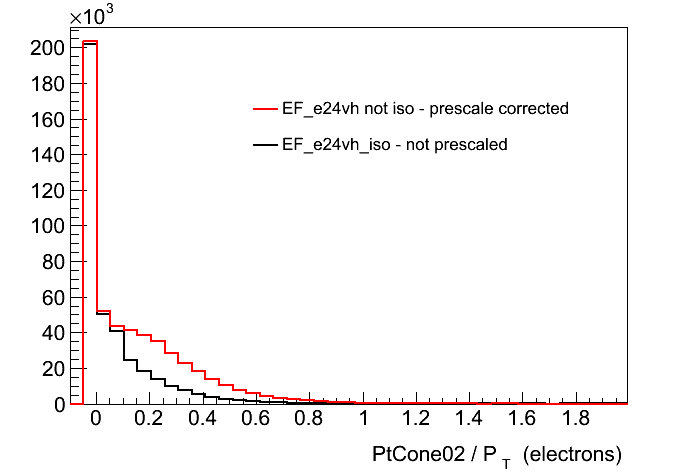
\includegraphics[width=9cm]{figure/appendix/trigger_comp.png}
\end{center}
\caption{\ptcone / \PT distribution for the analysis standard trigger and  its corrispective without isolation requirement,
this second trigger is rescaled according to prescales information.} 
\label{fig:prescale}
\end{figure}

\begin{figure}[t]
\begin{center}
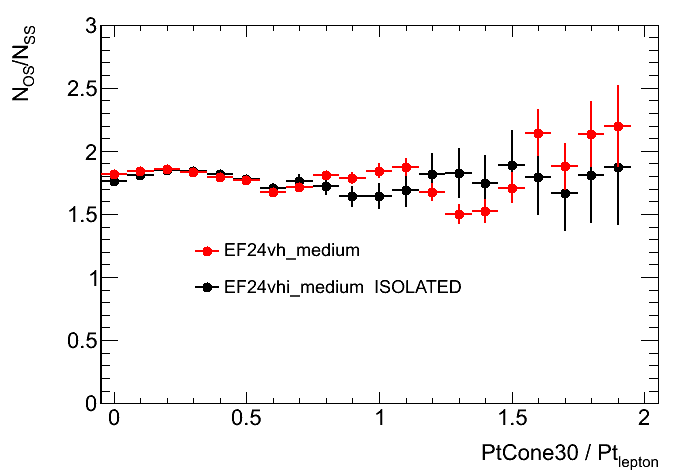
\includegraphics[width=0.49\textwidth]{figure/appendix/trig_comp_ptcone3.png}
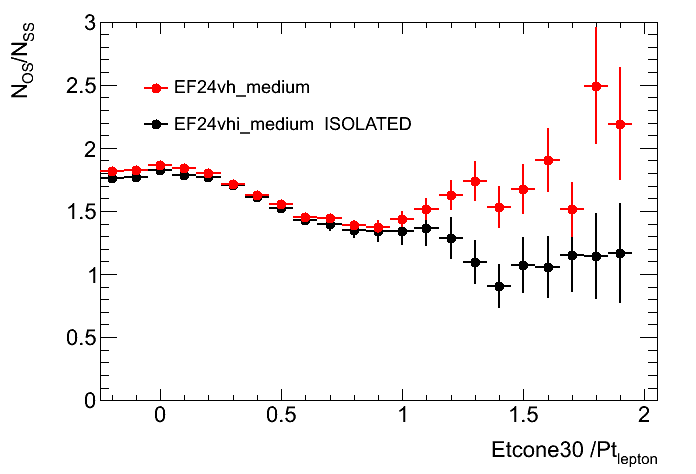
\includegraphics[width=0.49\textwidth]{figure/appendix/trig_comp_etcone3.png}
\end{center}
\caption{\rqcd  as a function of (a) \ptcone / \PT and (b) \etcone /PT for the electron triggers with and without isolation requirement.} 
\label{fig:trigRatio}
\end{figure}

\clearpage

\section{QCD Additional Plots}
\label{appendix:qcd_additional}

\begin{figure}[h!]
\begin{center}
\subfigure[]{
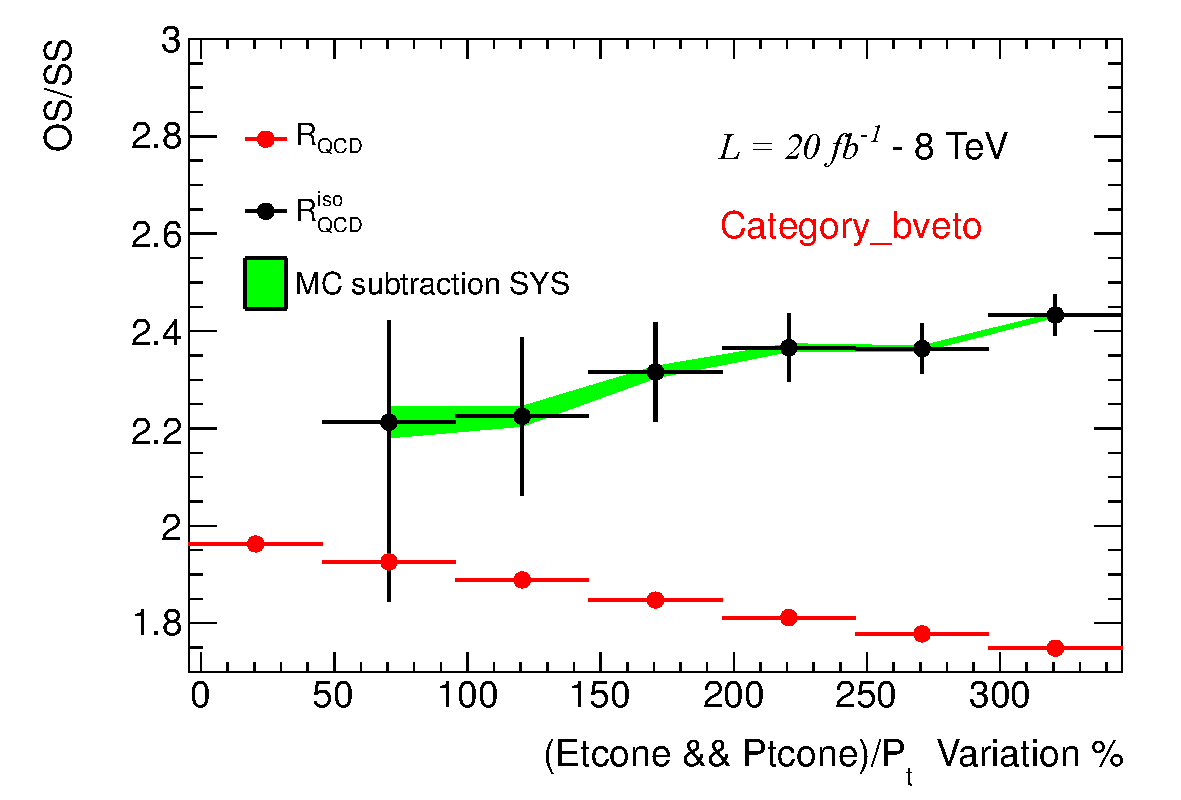
\includegraphics[width=0.45\textwidth]{figure/QCD/qcd_plot_1.pdf}
}
\subfigure[]{
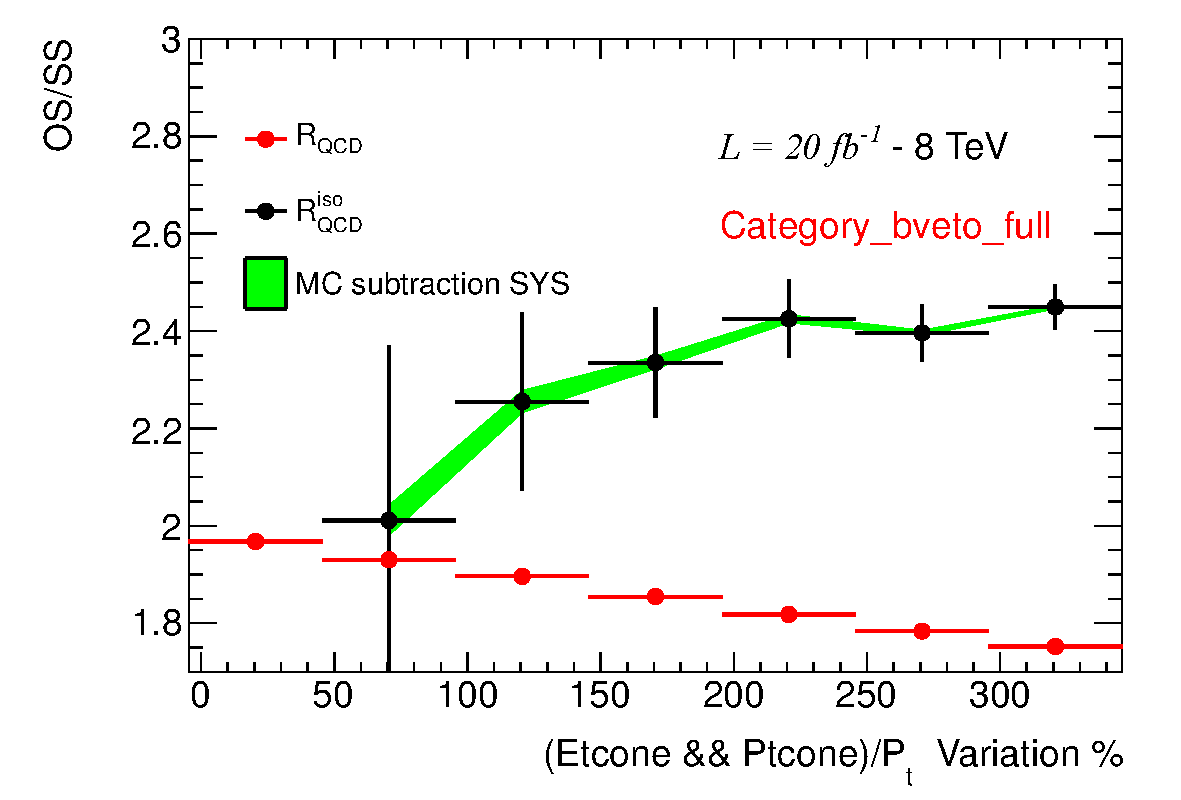
\includegraphics[width=0.45\textwidth]{figure/QCD/qcd_plot_2.pdf}
}
\subfigure[]{
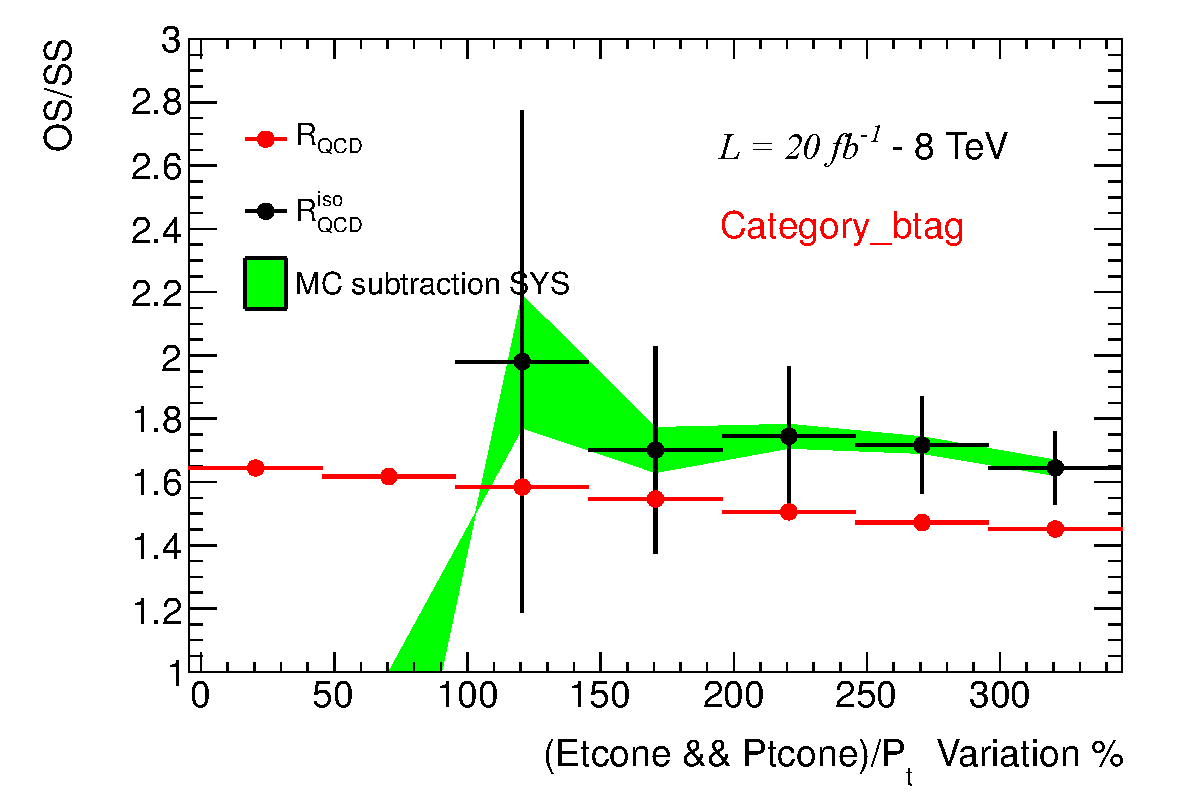
\includegraphics[width=0.45\textwidth]{figure/QCD/qcd_plot_4.pdf}
}
\subfigure[]{
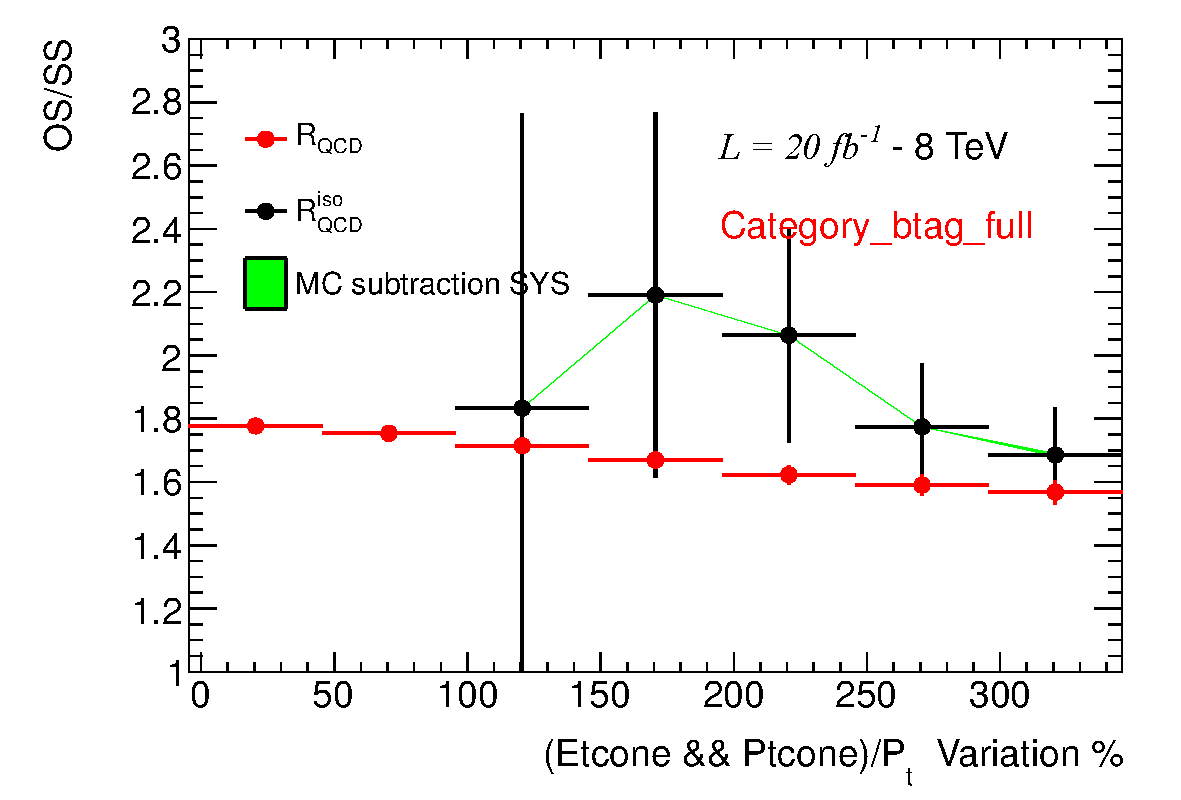
\includegraphics[width=0.45\textwidth]{figure/QCD/qcd_plot_3.pdf}
}
\end{center}
	\caption{OS/SS ratio as a function of lepton isolation variable selections after the requirement of (a) zero b-jets, (b) the full b-veto category selection, 
	(c) of a b-jet, (d) the full b-tag category selections. The isolation selections are varied as a percentage relative to
	the standard lepton isolation cut values (0~in the plot). 
	%As an example the point at 100\% in the plot corresponds
	%to $\rqcd$ evaluated by increasing the isolation requirement by 100\% respect to the standard cut value.
	The red points show the anti-isolated scale factor $\rqcd$, i.e. the ratio between regions C and D.
	 The black points show the isolated SF, which is defined as the ratio between region $\hat{A}$ and $\hat{B}$, 
	 where the leptons have isolation values larger than the nominal value but smaller
	 than the sliding cut.
%	 taking the same example point at 100\%, than the double of the standard cut value.
	 }
\end{figure}


